\documentclass[11pt]{article}
\usepackage{graphicx, subcaption}
\usepackage[top=1in, bottom=1in, left=1in, right=1in]{geometry}
\graphicspath{ {./figs/} }
\pagestyle{plain}
\def\changemargin#1#2{\list{}{\rightmargin#2\leftmargin#1}\item[]}
\let\endchangemargin=\endlist 
\begin{document}
\title{\vspace{-5mm}Comparison of $\kappa=1$ and $\kappa=0.5$}
\author{Alexander Holiday}
\date{}
\maketitle
\vspace{3cm}
\begin{changemargin}{0.0cm}{0.0cm}
\begin{figure}[h!]
  \vspace{-30mm}
  \begin{subfigure}{0.5\textwidth}
    \includegraphics[height=60mm]{n_500_2n3_3d_v2}
    \caption{$\kappa=0.5$}
    \label{fig:100s3}
  \end{subfigure}%
  \begin{subfigure}{0.5\textwidth}
    \includegraphics[height=60mm]{n_500_k_1_3d_2n3}
    \caption{$\kappa=1$}
    \label{fig:100s3}
  \end{subfigure}%
  \caption{Evolution of degrees. ($n=500$, $m=250000$)}
  \label{fig:n500_3d}
\end{figure}

\begin{figure}[h!]
  \vspace{-5mm}
  \centering
  \begin{subfigure}{0.5\textwidth}
    \centering
    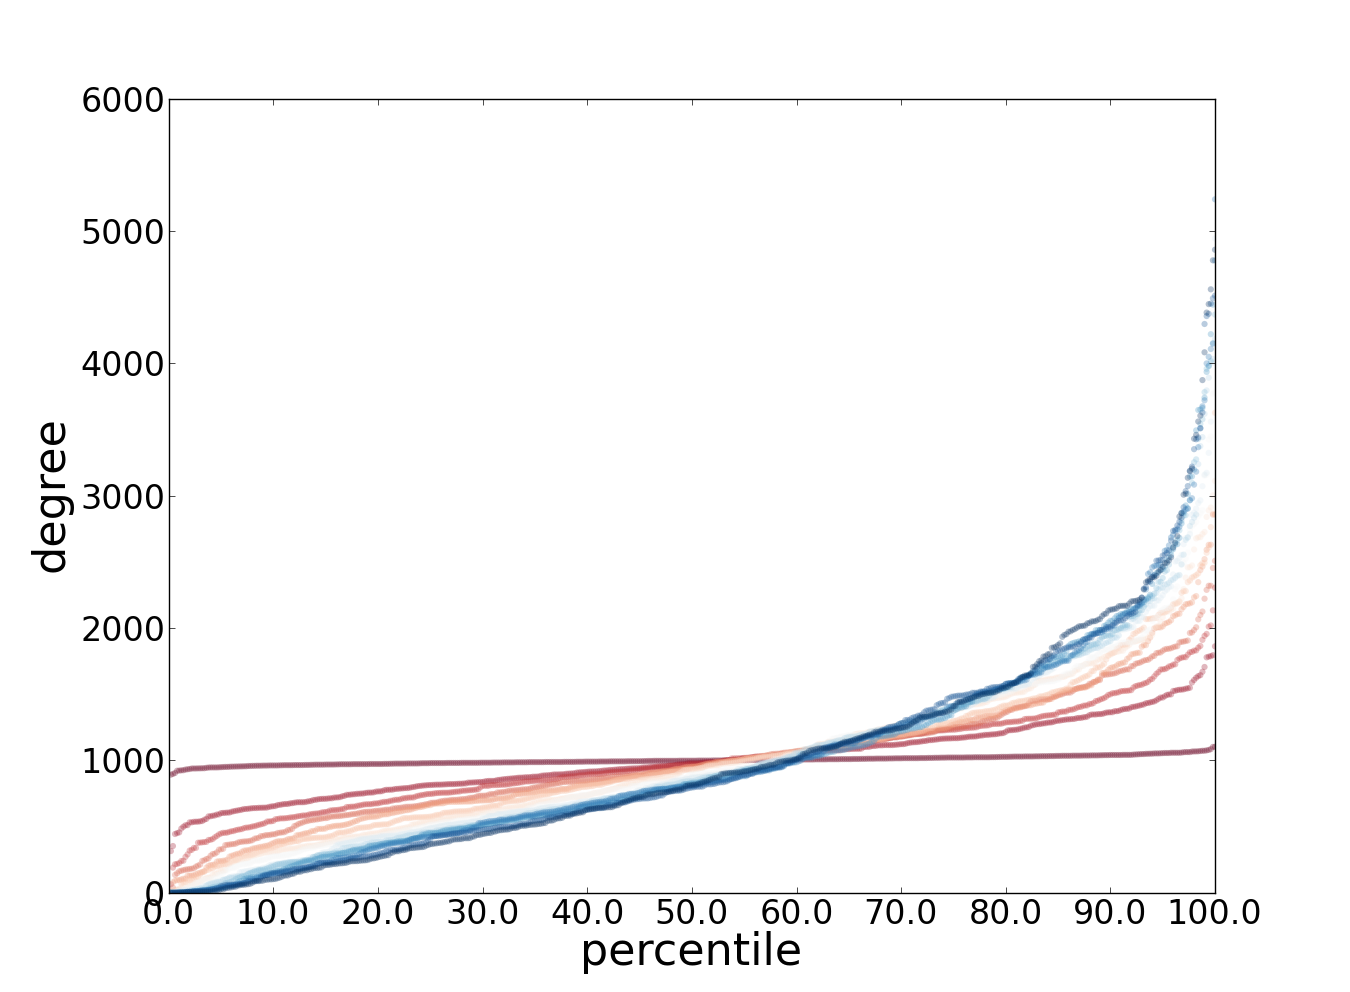
\includegraphics[height=60mm]{n_500_2n3_deg_percentile}
    \caption{$\kappa=0.5$}
    \label{fig:100s3}
  \end{subfigure}%
  \begin{subfigure}{0.5\textwidth}
    \centering
    \includegraphics[height=60mm]{n_500_k_1_deg_perc_2n3}
    \caption{$\kappa=1$}
    \label{fig:100s3}
  \end{subfigure}%
  \caption{Evolution of degrees and percentiles, a projection of Fig. \ref{fig:n500_3d} along the time axis. ($n=500$, $m=250000$)}
\end{figure}

\begin{figure}[h!]
  \vspace{-5mm}
  \centering
  \begin{subfigure}{0.5\textwidth}
    \centering
    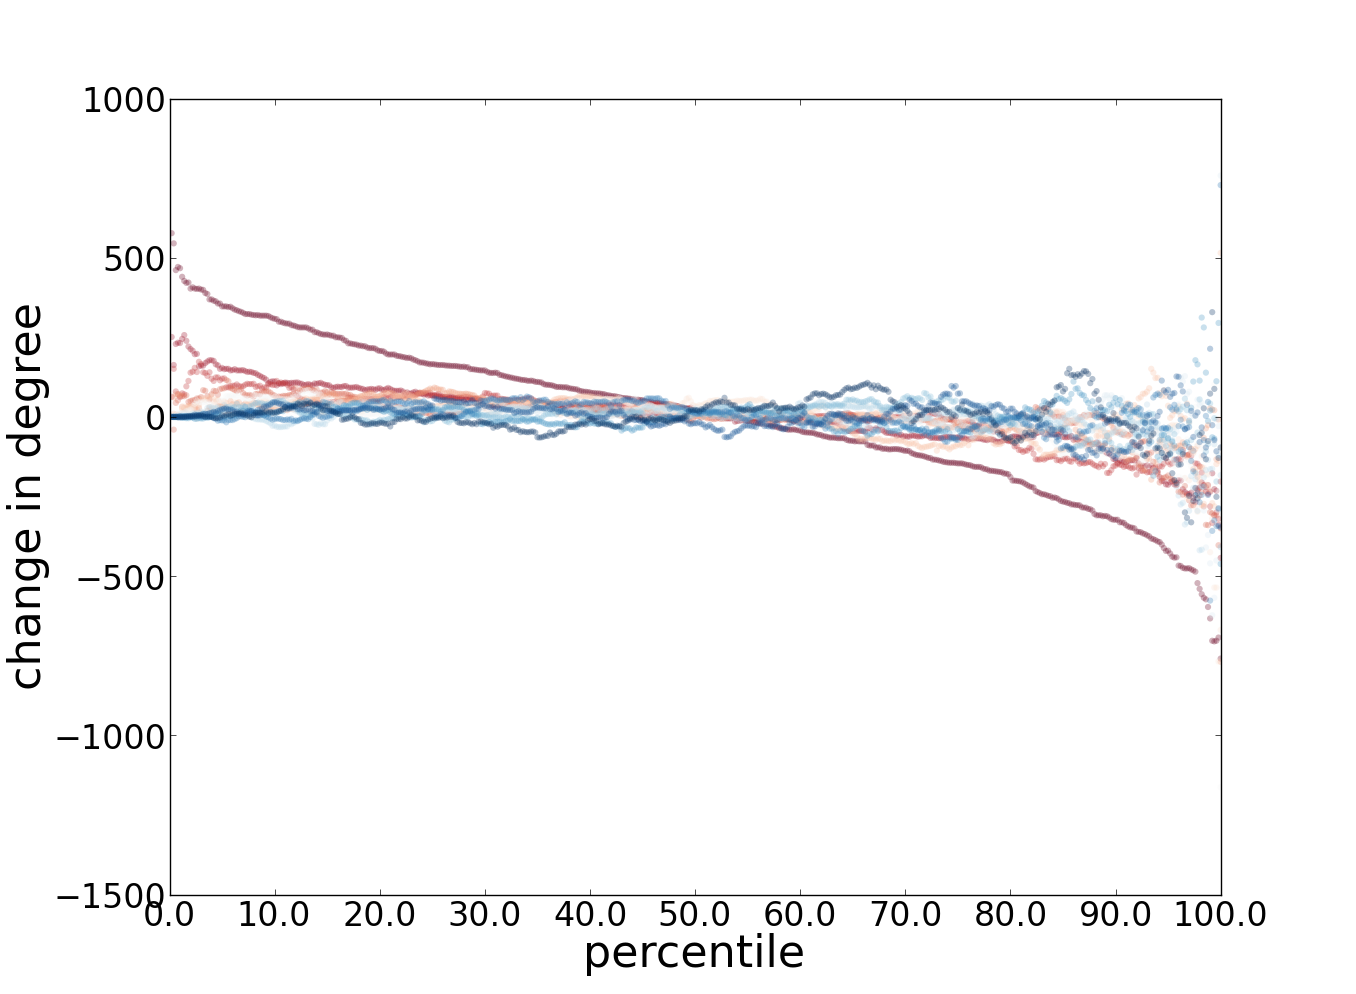
\includegraphics[height=60mm]{n_500_2n3_degchange_percentile}
    \caption{$\kappa=0.5$}
    \label{fig:100s3}
  \end{subfigure}%
  \begin{subfigure}{0.5\textwidth}
    \centering
    \includegraphics[height=60mm]{n_500_k_1_degchange_perc_2n3}
    \caption{$\kappa=1$}
    \label{fig:100s3}
  \end{subfigure}%
  \caption{Change in degree distribution between each step plotted against percentiles. ($n=500$, $m=250000$)}
\end{figure}

\begin{figure}[h!]
  \vspace{-5mm}
  \begin{subfigure}{0.5\textwidth}
    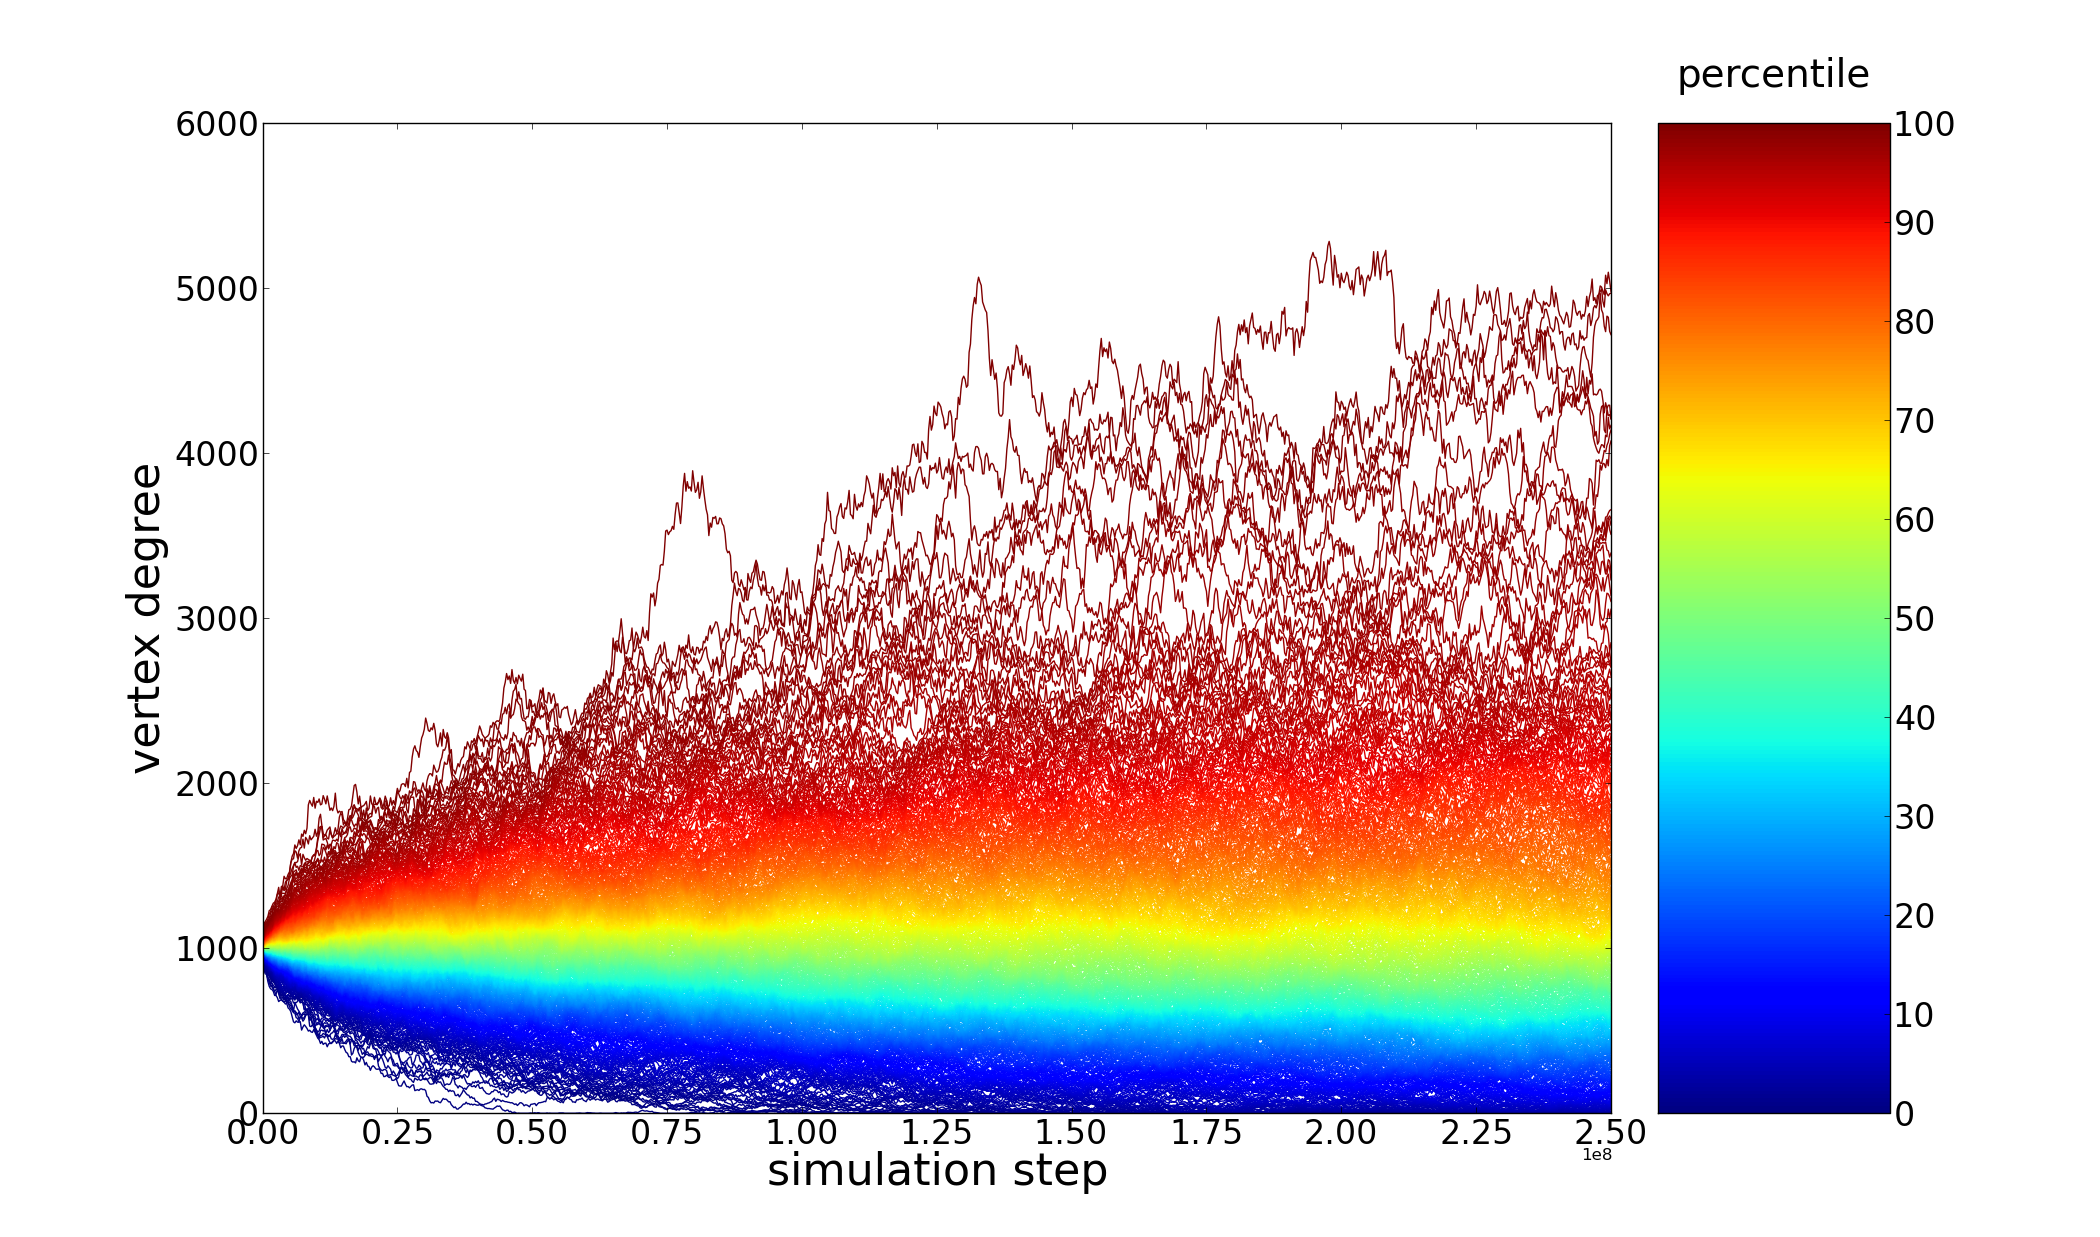
\includegraphics[height=50mm]{n_500_2n3_deg_step}
    \caption{$\kappa=0.5$}
    \label{fig:100s3}
  \end{subfigure}%
  \begin{subfigure}{0.5\textwidth}
    \includegraphics[height=50mm]{n_500_k_1_deg_step_2n3}
    \caption{$\kappa=1$}
    \label{fig:100s3}
  \end{subfigure}%
  \caption{Evolution of degree distribution. Color indicates percentile, e.g. the median degree at each step is colored green. ($n=500$, $m=250000$)}
\end{figure}
\end{changemargin}
\end{document}
